\documentclass{beamer}
\usepackage[utf8]{inputenc}
\usetheme{Madrid}
\usecolortheme{default}
\usepackage{amsmath,amssymb,amsfonts,amsthm}
\usepackage{txfonts}
\usepackage{tkz-euclide}
\usepackage{listings}
\usepackage{adjustbox}
\usepackage{array}
\usepackage{tabularx}
\usepackage{gvv}
\usepackage{lmodern}
\usepackage{circuitikz}
\usepackage{tikz}
\usepackage{graphicx}

\setbeamertemplate{page number in head/foot}[totalframenumber]

\usepackage{tcolorbox}
\tcbuselibrary{minted,breakable,xparse,skins}



\definecolor{bg}{gray}{0.95}
\DeclareTCBListing{mintedbox}{O{}m!O{}}{%
  breakable=true,
  listing engine=minted,
  listing only,
  minted language=#2,
  minted style=default,
  minted options={%
    linenos,
    gobble=0,
    breaklines=true,
    breakafter=,,
    fontsize=\small,
    numbersep=8pt,
    #1},
  boxsep=0pt,
  left skip=0pt,
  right skip=0pt,
  left=25pt,
  right=0pt,
  top=3pt,
  bottom=3pt,
  arc=5pt,
  leftrule=0pt,
  rightrule=0pt,
  bottomrule=2pt,
  toprule=2pt,
  colback=bg,
  colframe=orange!70,
  enhanced,
  overlay={%
    \begin{tcbclipinterior}
    \fill[orange!20!white] (frame.south west) rectangle ([xshift=20pt]frame.north west);
    \end{tcbclipinterior}},
  #3,
}
\lstset{
    language=C,
    basicstyle=\ttfamily\small,
    keywordstyle=\color{blue},
    stringstyle=\color{orange},
    commentstyle=\color{green!60!black},
    numbers=left,
    numberstyle=\tiny\color{gray},
    breaklines=true,
    showstringspaces=false,
}
%------------------------------------------------------------
%This block of code defines the information to appear in the
%Title page
\title %optional
{8.2.55}

%\subtitle{A short story}

\author % (optional)
{BALU-ai25btech11017}



\begin{document}


\frame{\titlepage}
\begin{frame}{Question}
Equation of the hyperbola with eccentricity \( \frac{3}{2} \) and foci at \( (\pm 2, 0) \) is \underline{\hspace{3cm}}.
\\ 
\end{frame}
\begin{frame}{Theoretical Solution}
Let us solve the given equation theoretically and then verify the solution computationally \\
According to the question, \\
\begin{align}
e=\frac{3}{2}\
\vec{F_1}=\myvec{2\\0}\
\vec{F_2}=\myvec{-2\\0}\\
\vec{n}=\vec{F_1}-\vec{F_2}=\myvec{4\\0}\\
\vec{n}^T\vec{x}=c\
\end{align}
hyperbola equation is\\
\begin{align}
   \vec{x}^T\vec{v}\vec{x}+2\vec{u}^T\vec{x}+f=0
\end{align}
\begin{align}
   \vec{v}=\|\vec{n}\|^2\vec{I}-e^2\vec{n}\vec{n}^T\\
   \vec{u}=ce^2\vec{e_1}-\vec{F}\
   \end{align}
\end{frame}
\begin{frame}{Theoretical Solution}
\begin{align}
   f=\|\vec{n}\|^2\|\vec{F}\|^2-c^2e^2
\end{align}
\begin{align}
    \vec{u}=\frac{\vec{F_1}+\vec{F_2}}{2}=\myvec{0\\0}\\
    \vec{v}=\myvec{-20&&0\\0&&16}\\
    f=60\
\end{align}
hence the requried hyperbola equation is
\begin{align}
   \vec{x}^T\myvec{-20&&0\\0&&16}\vec{x}+60=0
\end{align}
\end{frame}
\begin{frame}[fragile]
    \frametitle{C Code}

    \begin{lstlisting}
 #include <stdio.h>
#include <math.h>

int main() {
    // Given
    double e = 1.5;   // eccentricity
    double c = 2.0;   // focus distance

    // Compute parameters
    double a = c / e;       // semi-major axis
    double b2 = c*c - a*a;  // b^2
    double b = sqrt(b2);

    // Conic form coefficients (for Python V, u, f)
    double V11 = 9.0/16.0;
    double V22 = -9.0/20.0;
    double f   = -1.0;

  

  

    \end{lstlisting}
\end{frame}
\begin{frame}[fragile]
    \frametitle{C Code }
    \begin{lstlisting}
    // Output in Python-readable format
    printf("# Hyperbola parameters\n");
    printf("a = %.6f\n", a);
    printf("b = %.6f\n", b);
    printf("V = [[%.6f, 0], [0, %.6f]]\n", V11, V22);
    printf("u = [[0], [0]]\n");
    printf("f = %.1f\n", f);

    return 0;
}
    \end{lstlisting}
\end{frame}
\begin{frame}[fragile]
    \frametitle{python Code }
    \begin{lstlisting}
#Program to plot a hyperbola 
#Code by GVV Sharma (Modified)
#Updated: Sep 2025

import numpy as np
import matplotlib.pyplot as plt
from numpy import linalg as LA
import sys

# For path to external scripts
sys.path.insert(0, '/sdcard/github/matgeo/codes/CoordGeo')

# Local imports
from line.funcs import *
from triangle.funcs import *
from conics.funcs import *












  \end{lstlisting}
\end{frame}
\begin{frame}[fragile]
    \frametitle{python Code }
    \begin{lstlisting}
# Plotting setup
fig = plt.figure()
ax = fig.add_subplot(111, aspect='equal')
len = 100
y = np.linspace(-2, 2, len)

#-----------------------------------
# Hyperbola Parameters from Question
# Eccentricity e = 3/2
# Foci at (±2, 0) ⇒ c = 2 ⇒ a = 4/3, b^2 = c^2 - a^2 = 20/9

a = 4 / 3
b = np.sqrt(20 / 9)

# Conic form: (x^2 / a^2) - (y^2 / b^2) = 1
# Multiply both sides to get general quadratic: 
# (9x^2 / 16) - (9y^2 / 20) = 1
# ⇒ V matrix, u vector, f scalar such that x^T V x + f = 0

\end{lstlisting}
\end{frame}
\begin{frame}[fragile]
    \frametitle{python Code }
    \begin{lstlisting}
V = np.array([[9/16, 0], [0, -9/20]])
u = np.array([[0], [0]])
f = -1

# Get conic parameters using your utility function
n, c, F, O, lam, P, e = conic_param(V, u, f)

# Affine transform matrix (diagonal since axes aligned)
ParamMatrix = np.diag([a, b])

# Generate standard hyperbola
x = hyper_gen(y)
xStandardHyperLeft = np.block([[-x], [y]])
xStandardHyperRight = np.block([[x], [y]])

# Apply affine transform
Of = O.flatten()
xActualHyperLeft = P @ ParamMatrix @ xStandardHyperLeft + Of[:, np.newaxis]
    \end{lstlisting}
\end{frame}
\begin{frame}[fragile]
    \frametitle{python Code }
    \begin{lstlisting}
xActualHyperRight = P @ ParamMatrix @ xStandardHyperRight + Of[:, np.newaxis]

# Directrix and Latus Rectum lines
k1 = -2
k2 = 2
cl = (n.T @ F).flatten()

x_A = line_norm(n, c[0], k1, k2)   # Left directrix
x_B = line_norm(n, cl[0], k1, k2) # Left latus rectum
x_C = line_norm(n, c[1], k1, k2)  # Right directrix
x_D = line_norm(n, cl[1], k1, k2) # Right latus rectum

# Plotting
plt.plot(xActualHyperLeft[0, :], xActualHyperLeft[1, :], label='Hyperbola', color='r')
plt.plot(xActualHyperRight[0, :], xActualHyperRight[1, :], color='r')
     \end{lstlisting}
\end{frame}
\begin{frame}[fragile]
    \frametitle{python Code }
    \begin{lstlisting}
plt.plot(x_A[0, :], x_A[1, :], label='Directrix')
plt.plot(x_B[0, :], x_B[1, :], label='Latus Rectum')
plt.plot(x_C[0, :], x_C[1, :])
plt.plot(x_D[0, :], x_D[1, :])

# Plot origin and foci
tri_coords = np.block([O, F])
plt.scatter(tri_coords[0, :], tri_coords[1, :], c=np.arange(1, 4))
vert_labels = ['$\mathbf{O}$', '$\mathbf{F}_1$', '$\mathbf{F}_2$']
for i, txt in enumerate(vert_labels):
    plt.annotate(txt, (tri_coords[0, i], tri_coords[1, i]), 
                 textcoords="offset points", xytext=(-10, 5), ha='center')
    \end{lstlisting}
\end{frame}
\begin{frame}[fragile]
    \frametitle{python Code }
    \begin{lstlisting}
# Axes formatting
ax = plt.gca()
ax.spines['top'].set_color('none')
ax.spines['left'].set_position('zero')
ax.spines['right'].set_color('none')
ax.spines['bottom'].set_position('zero')
plt.xlabel('$x$')
plt.ylabel('$y$')
plt.legend(loc='best')
plt.grid()
plt.axis('equal')
# For Termux
plt.savefig('chapters/11/11/4/13/figs/fig.pdf')
import subprocess
import shlex
subprocess.run(shlex.split("termux-open chapters/11/11/4/13/figs/fig.pdf"))
# Otherwise uncomment to show plot
# plt.show()
     \end{lstlisting}
\end{frame}
\begin{frame}{Plot}
    \centering
    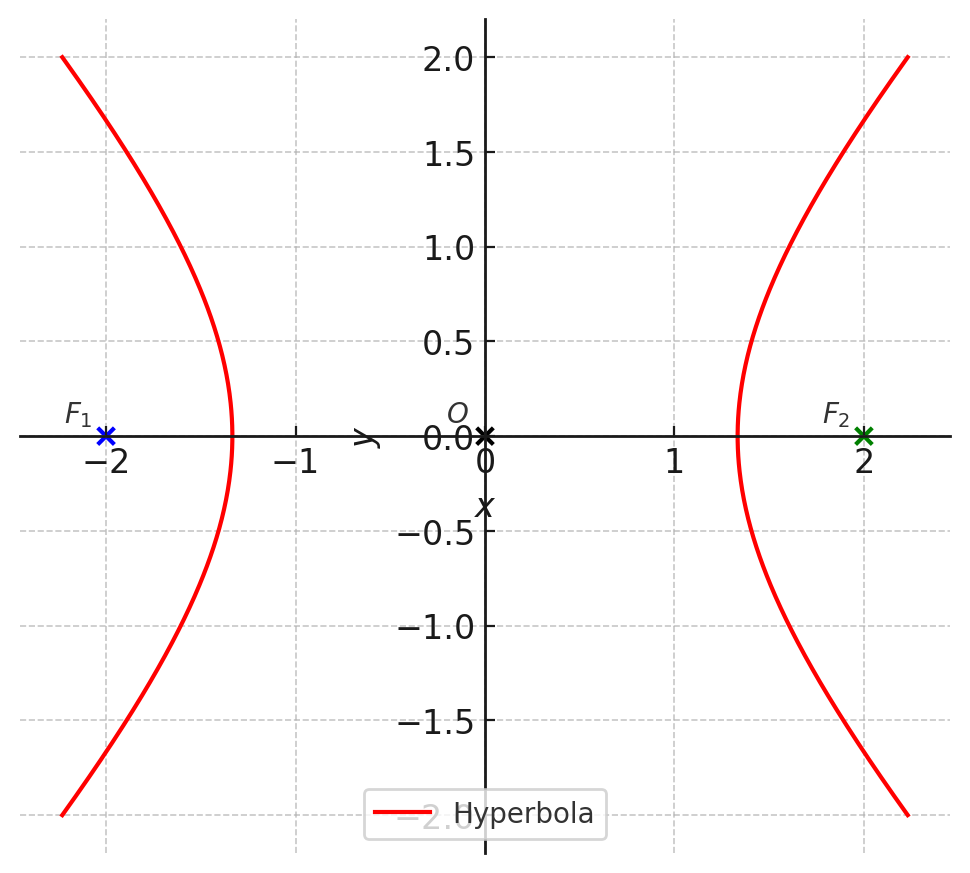
\includegraphics[width=\columnwidth, height=0.8\textheight, keepaspectratio]{figs/hyperbola.png}     
\end{frame}
\end{document}